% Options for packages loaded elsewhere
\PassOptionsToPackage{unicode}{hyperref}
\PassOptionsToPackage{hyphens}{url}
\PassOptionsToPackage{dvipsnames,svgnames,x11names}{xcolor}
%
\documentclass[
  letterpaper,
  DIV=11,
  numbers=noendperiod]{scrartcl}

\usepackage{amsmath,amssymb}
\usepackage{iftex}
\ifPDFTeX
  \usepackage[T1]{fontenc}
  \usepackage[utf8]{inputenc}
  \usepackage{textcomp} % provide euro and other symbols
\else % if luatex or xetex
  \usepackage{unicode-math}
  \defaultfontfeatures{Scale=MatchLowercase}
  \defaultfontfeatures[\rmfamily]{Ligatures=TeX,Scale=1}
\fi
\usepackage{lmodern}
\ifPDFTeX\else  
    % xetex/luatex font selection
\fi
% Use upquote if available, for straight quotes in verbatim environments
\IfFileExists{upquote.sty}{\usepackage{upquote}}{}
\IfFileExists{microtype.sty}{% use microtype if available
  \usepackage[]{microtype}
  \UseMicrotypeSet[protrusion]{basicmath} % disable protrusion for tt fonts
}{}
\makeatletter
\@ifundefined{KOMAClassName}{% if non-KOMA class
  \IfFileExists{parskip.sty}{%
    \usepackage{parskip}
  }{% else
    \setlength{\parindent}{0pt}
    \setlength{\parskip}{6pt plus 2pt minus 1pt}}
}{% if KOMA class
  \KOMAoptions{parskip=half}}
\makeatother
\usepackage{xcolor}
\setlength{\emergencystretch}{3em} % prevent overfull lines
\setcounter{secnumdepth}{-\maxdimen} % remove section numbering
% Make \paragraph and \subparagraph free-standing
\makeatletter
\ifx\paragraph\undefined\else
  \let\oldparagraph\paragraph
  \renewcommand{\paragraph}{
    \@ifstar
      \xxxParagraphStar
      \xxxParagraphNoStar
  }
  \newcommand{\xxxParagraphStar}[1]{\oldparagraph*{#1}\mbox{}}
  \newcommand{\xxxParagraphNoStar}[1]{\oldparagraph{#1}\mbox{}}
\fi
\ifx\subparagraph\undefined\else
  \let\oldsubparagraph\subparagraph
  \renewcommand{\subparagraph}{
    \@ifstar
      \xxxSubParagraphStar
      \xxxSubParagraphNoStar
  }
  \newcommand{\xxxSubParagraphStar}[1]{\oldsubparagraph*{#1}\mbox{}}
  \newcommand{\xxxSubParagraphNoStar}[1]{\oldsubparagraph{#1}\mbox{}}
\fi
\makeatother


\providecommand{\tightlist}{%
  \setlength{\itemsep}{0pt}\setlength{\parskip}{0pt}}\usepackage{longtable,booktabs,array}
\usepackage{calc} % for calculating minipage widths
% Correct order of tables after \paragraph or \subparagraph
\usepackage{etoolbox}
\makeatletter
\patchcmd\longtable{\par}{\if@noskipsec\mbox{}\fi\par}{}{}
\makeatother
% Allow footnotes in longtable head/foot
\IfFileExists{footnotehyper.sty}{\usepackage{footnotehyper}}{\usepackage{footnote}}
\makesavenoteenv{longtable}
\usepackage{graphicx}
\makeatletter
\newsavebox\pandoc@box
\newcommand*\pandocbounded[1]{% scales image to fit in text height/width
  \sbox\pandoc@box{#1}%
  \Gscale@div\@tempa{\textheight}{\dimexpr\ht\pandoc@box+\dp\pandoc@box\relax}%
  \Gscale@div\@tempb{\linewidth}{\wd\pandoc@box}%
  \ifdim\@tempb\p@<\@tempa\p@\let\@tempa\@tempb\fi% select the smaller of both
  \ifdim\@tempa\p@<\p@\scalebox{\@tempa}{\usebox\pandoc@box}%
  \else\usebox{\pandoc@box}%
  \fi%
}
% Set default figure placement to htbp
\def\fps@figure{htbp}
\makeatother
% definitions for citeproc citations
\NewDocumentCommand\citeproctext{}{}
\NewDocumentCommand\citeproc{mm}{%
  \begingroup\def\citeproctext{#2}\cite{#1}\endgroup}
\makeatletter
 % allow citations to break across lines
 \let\@cite@ofmt\@firstofone
 % avoid brackets around text for \cite:
 \def\@biblabel#1{}
 \def\@cite#1#2{{#1\if@tempswa , #2\fi}}
\makeatother
\newlength{\cslhangindent}
\setlength{\cslhangindent}{1.5em}
\newlength{\csllabelwidth}
\setlength{\csllabelwidth}{3em}
\newenvironment{CSLReferences}[2] % #1 hanging-indent, #2 entry-spacing
 {\begin{list}{}{%
  \setlength{\itemindent}{0pt}
  \setlength{\leftmargin}{0pt}
  \setlength{\parsep}{0pt}
  % turn on hanging indent if param 1 is 1
  \ifodd #1
   \setlength{\leftmargin}{\cslhangindent}
   \setlength{\itemindent}{-1\cslhangindent}
  \fi
  % set entry spacing
  \setlength{\itemsep}{#2\baselineskip}}}
 {\end{list}}
\usepackage{calc}
\newcommand{\CSLBlock}[1]{\hfill\break\parbox[t]{\linewidth}{\strut\ignorespaces#1\strut}}
\newcommand{\CSLLeftMargin}[1]{\parbox[t]{\csllabelwidth}{\strut#1\strut}}
\newcommand{\CSLRightInline}[1]{\parbox[t]{\linewidth - \csllabelwidth}{\strut#1\strut}}
\newcommand{\CSLIndent}[1]{\hspace{\cslhangindent}#1}

\KOMAoption{captions}{tableheading}
\makeatletter
\@ifpackageloaded{caption}{}{\usepackage{caption}}
\AtBeginDocument{%
\ifdefined\contentsname
  \renewcommand*\contentsname{Table of contents}
\else
  \newcommand\contentsname{Table of contents}
\fi
\ifdefined\listfigurename
  \renewcommand*\listfigurename{List of Figures}
\else
  \newcommand\listfigurename{List of Figures}
\fi
\ifdefined\listtablename
  \renewcommand*\listtablename{List of Tables}
\else
  \newcommand\listtablename{List of Tables}
\fi
\ifdefined\figurename
  \renewcommand*\figurename{Figure}
\else
  \newcommand\figurename{Figure}
\fi
\ifdefined\tablename
  \renewcommand*\tablename{Table}
\else
  \newcommand\tablename{Table}
\fi
}
\@ifpackageloaded{float}{}{\usepackage{float}}
\floatstyle{ruled}
\@ifundefined{c@chapter}{\newfloat{codelisting}{h}{lop}}{\newfloat{codelisting}{h}{lop}[chapter]}
\floatname{codelisting}{Listing}
\newcommand*\listoflistings{\listof{codelisting}{List of Listings}}
\makeatother
\makeatletter
\makeatother
\makeatletter
\@ifpackageloaded{caption}{}{\usepackage{caption}}
\@ifpackageloaded{subcaption}{}{\usepackage{subcaption}}
\makeatother

\usepackage{bookmark}

\IfFileExists{xurl.sty}{\usepackage{xurl}}{} % add URL line breaks if available
\urlstyle{same} % disable monospaced font for URLs
\hypersetup{
  pdftitle={Modelling complex traits with ancestral recombination graphs},
  pdfauthor={Hanbin Lee},
  colorlinks=true,
  linkcolor={blue},
  filecolor={Maroon},
  citecolor={Blue},
  urlcolor={Blue},
  pdfcreator={LaTeX via pandoc}}


\title{Modelling complex traits with ancestral recombination graphs}
\author{Hanbin Lee}
\date{Mar 7, 2025}

\begin{document}
\maketitle


\section{Overview}\label{overview}

The ancestral recombination graph (ARG) describes the evolutionary
relationship between

genetic materials in the presence of recombination and drift

\begin{figure}[H]

{\centering 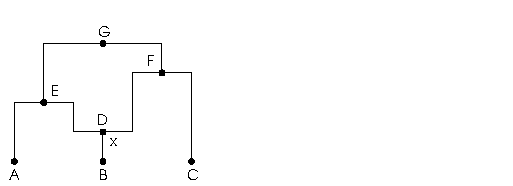
\includegraphics[width=\linewidth,height=6.25in,keepaspectratio]{slides_files/mediabag/imgs/full_arg-0.pdf}

}

\caption{From (Wong et al. 2024)}

\end{figure}%

The ancestral recombination graph (ARG) describes the evolutionary
relationship between

genetic materials in the presence of recombination and drift

\begin{figure}[H]

{\centering 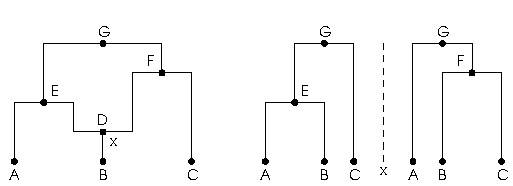
\includegraphics[width=\linewidth,height=6.25in,keepaspectratio]{slides_files/mediabag/imgs/full_arg-1.pdf}

}

\caption{From (Wong et al. 2024)}

\end{figure}%

The full probabilistic process is complicated

In this work, we condition on the realized ARG, resulting a sequence of
local trees

\begin{figure}[H]

{\centering 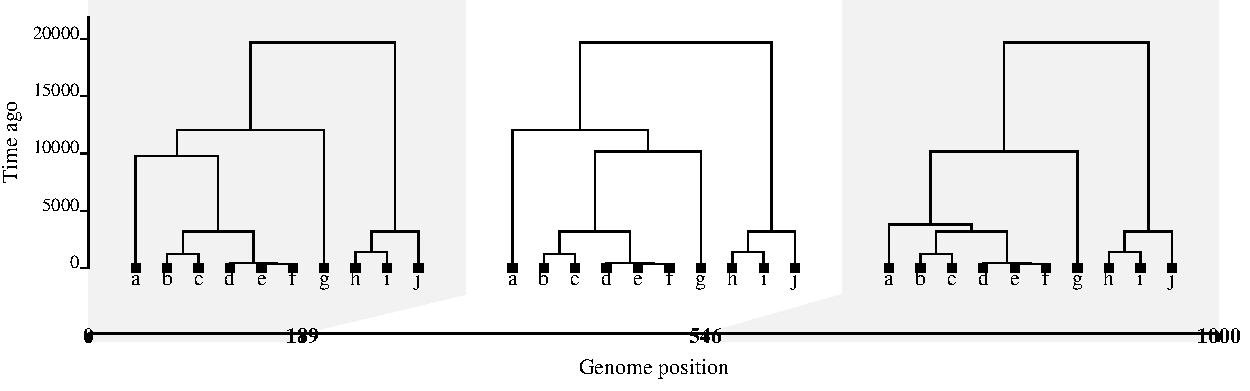
\includegraphics[width=\linewidth,height=5.20833in,keepaspectratio]{slides_files/mediabag/imgs/local_trees.pdf}

}

\caption{From \href{https://tskit.dev/tutorials/what_is.html}{tskit
docs}}

\end{figure}%

What is the conditional distribution of a trait given the trees?

Since the genealogy is fixed, the only randomness that remains is
mutation

\[
\text{Trait} \mid \text{Local trees} \quad \sim \quad ?
\]

\subsection{Linear mixed model}\label{linear-mixed-model}

Linear mixed models are popular in quantitative genetics \[
\mathbf{y} = \underbrace{\mathbf{Z}\mathbf{u}}_{\text{random effects}} + \underbrace{\mathbf{X}\mathbf{b}}_{\text{fixed effects}} + \boldsymbol{\varepsilon}
\] where \(\mathbf{Z}\) includes genotyped variants and \(\mathbf{X}\)
is the covariate matrix

In particular, the SNP effects \(\mathbf{u} \sim p(\cdot)\) is
\emph{random}

Some questions \ldots{}

\begin{itemize}
\tightlist
\item
  What's the source of \(\mathbf{u}\)'s randomness?
\item
  Why are \(\mathbf{u}\)'s (vector of random effects) entries
  independent?
\end{itemize}

We answer these questions from a genealogical perspective

\section{Setup and derivation}\label{setup-and-derivation}

The trait \(\mathbf{y}\) is a linear function of the genotype
\(\mathbf{G}\) \[
\mathbf{y} = \mathbf{G}\boldsymbol{\beta} + \boldsymbol{\varepsilon}
\] \(\mathbf{y} \in \mathbb{R}^N\),
\(\mathbf{G} \in \mathbb{R}^{N \times P}\),
\(\boldsymbol{\beta} \in \mathbb{R}^P\), and
\(\boldsymbol{\varepsilon} \in \mathbb{R}^N\)

\(\mathbf{G}\) contains \emph{all} positions the genome including
genotyped ones

\(N\): number of samples, \(P\): length of the genome

\subsection{How do we get traits?}\label{how-do-we-get-traits}

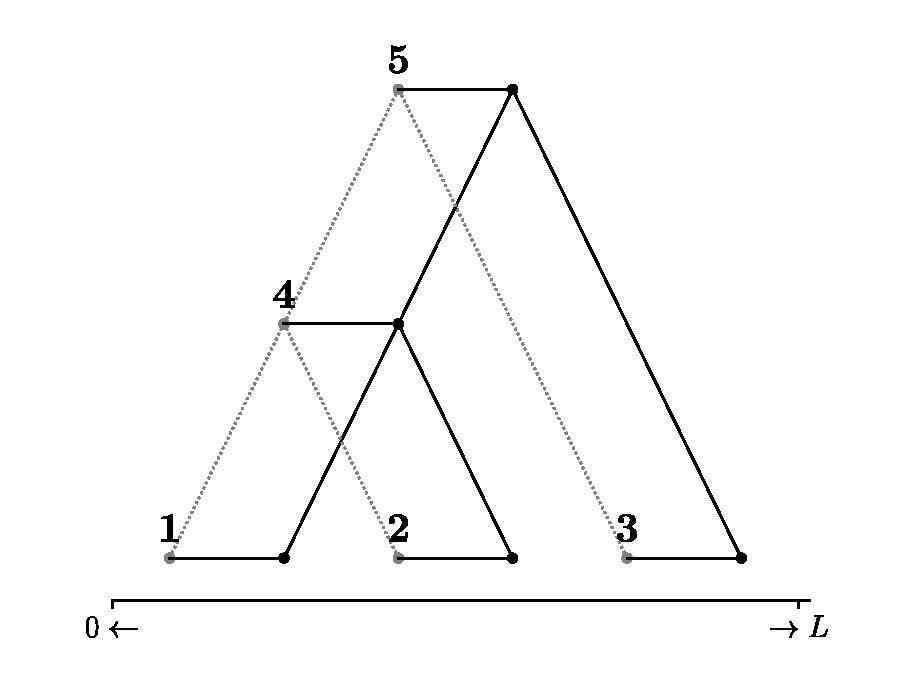
\includegraphics[width=\linewidth,height=6.25in,keepaspectratio]{slides_files/mediabag/imgs/tree-branch.pdf}

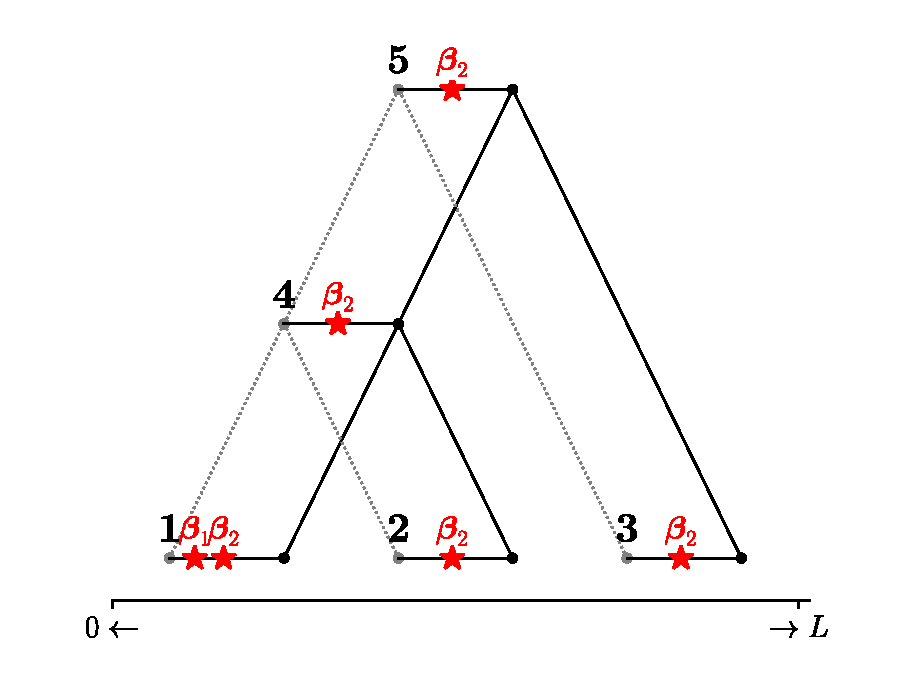
\includegraphics[width=\linewidth,height=6.25in,keepaspectratio]{slides_files/mediabag/imgs/tree-0.pdf}
\[
\mathbf{y}_1=\boldsymbol{\beta}_1+\boldsymbol{\beta}_2, \;
\mathbf{y}_2 = \boldsymbol{\beta}_2, \;
\mathbf{y}_3 = \boldsymbol{\beta}_2
\]

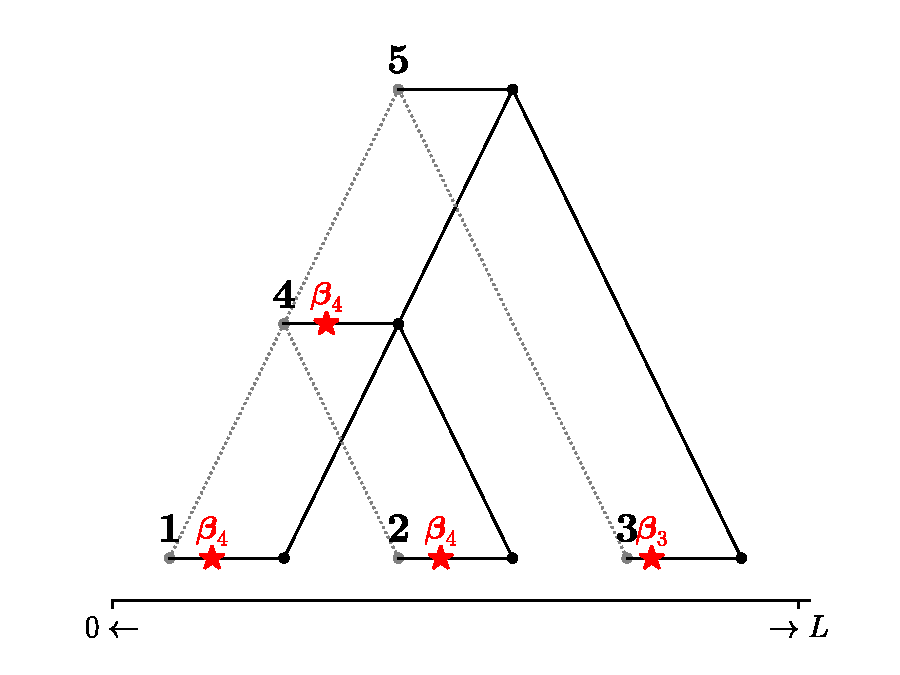
\includegraphics[width=\linewidth,height=6.25in,keepaspectratio]{slides_files/mediabag/imgs/tree-1.pdf}
\[
\mathbf{y}_1=\boldsymbol{\beta}_4, \;
\mathbf{y}_2=\boldsymbol{\beta}_4, \;
\mathbf{y}_3 = \boldsymbol{\beta}_3
\]

Consider a local tree that spans over a region

We get trait values by adding up effect sizes (\(\boldsymbol{\beta}\))

\begin{itemize}
\tightlist
\item
  \(\mathbf{y}_n = \mathbf{G}_{n1} \boldsymbol{\beta}_1 + \mathbf{G}_{n2} \boldsymbol{\beta}_2\)
\end{itemize}

\begin{itemize}
\tightlist
\item
  \(\mathbf{y}_n = \mathbf{G}_{n3} \boldsymbol{\beta}_3 + \mathbf{G}_{n4} \boldsymbol{\beta}_4\)
\end{itemize}

\subsection{Branch-centric view of trait
transmission}\label{branch-centric-view-of-trait-transmission}

\begin{center}
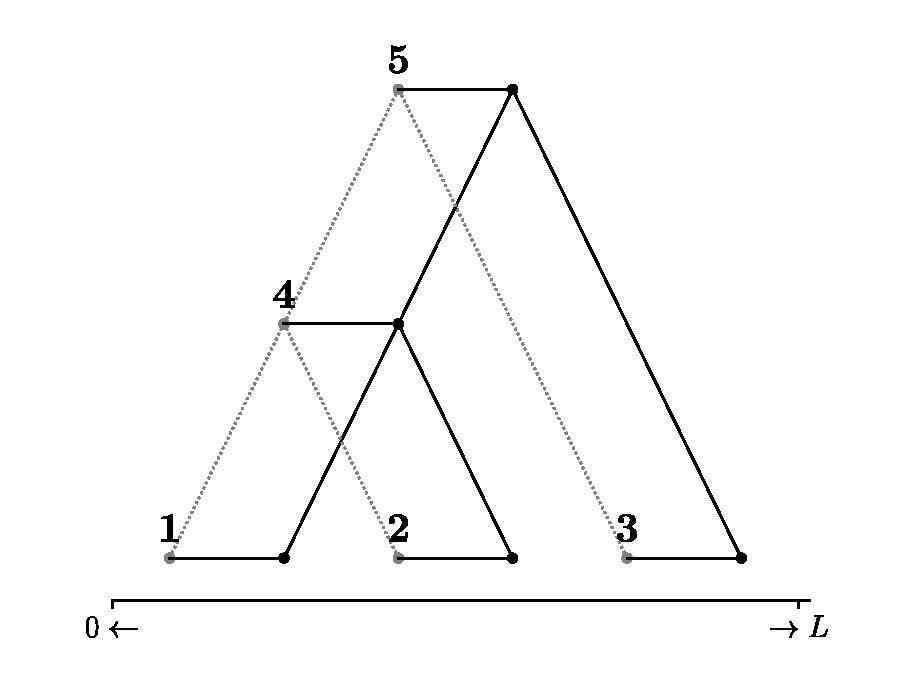
\includegraphics[width=\linewidth,height=6.25in,keepaspectratio]{slides_files/mediabag/imgs/tree-branch.pdf}
\end{center}

\begin{center}
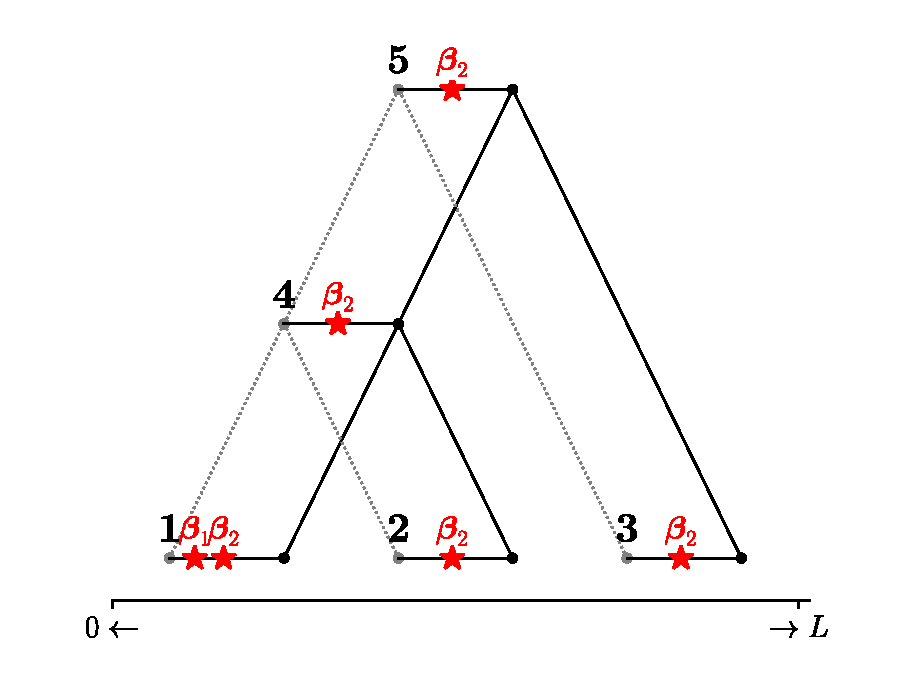
\includegraphics[width=\linewidth,height=6.25in,keepaspectratio]{slides_files/mediabag/imgs/tree-0.pdf}
\end{center}

\begin{center}
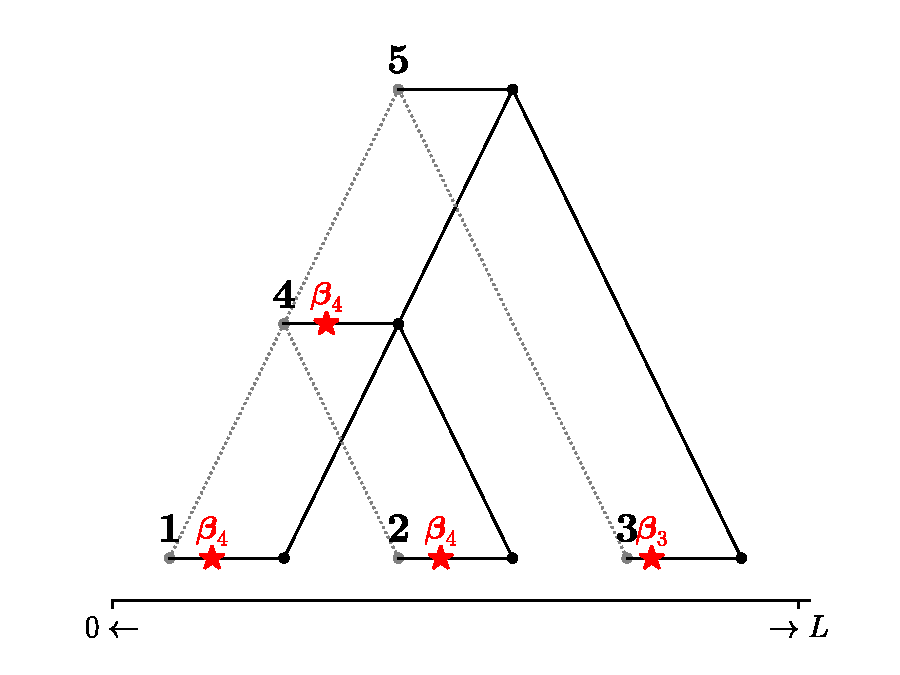
\includegraphics[width=\linewidth,height=6.25in,keepaspectratio]{slides_files/mediabag/imgs/tree-1.pdf}
\end{center}

Inherit a branch first, then a mutation

\begin{itemize}
\tightlist
\item
  Sample \(1\) inherits edges \(1-4\) and \(4-5\)
\end{itemize}

\begin{itemize}
\tightlist
\item
  Sample \(2\) inherits edges \(2-4\) and \(4-5\)
\end{itemize}

\begin{itemize}
\tightlist
\item
  Sample \(3\) inherits edge \(3-5\)
\end{itemize}

Branch's effect \(=\) Sum of mutations' effect

\begin{itemize}
\tightlist
\item
  Effect of \(4-5 = 0\) (1st realization)
\end{itemize}

\begin{itemize}
\tightlist
\item
  Effect of \(4-5 = \boldsymbol{\beta}_4\) (2nd realization)
\end{itemize}

Branch effect is a random variable!

\subsection{From variants to branches}\label{from-variants-to-branches}

\[
\text{Trait} = \sum_p \text{Variant$_p$ effect size} 
\quad
\Rightarrow 
\quad
\text{Trait} = \sum_e \text{Branch$_e$ effect size}
\]

\[
\boldsymbol{\upsilon}_e = \text{Branch$_e$ effect size} = \sum_p \text{Variant$_p$ on Branch$_e$}
\]

\[
\mathbf{y} = \sum_p \mathbf{G}_p\boldsymbol{\beta}_p + \boldsymbol{\varepsilon}
\quad
\Rightarrow
\quad
\mathbf{y} = \sum_e \mathbf{Z}_e\boldsymbol{\upsilon}_e + \boldsymbol{\varepsilon} 
\] where \(\mathbf{Z}_{ne}=\) the number of haplotypes of \(n\) that
inherit \(e\)

\section{Ancestral recombination graph linear mixed model
(ARG-LMM)}\label{ancestral-recombination-graph-linear-mixed-model-arg-lmm}

Split \(\boldsymbol{\upsilon}\) to
\(\mathbf{u} = \boldsymbol{\upsilon} - \mathrm{E}\boldsymbol{\upsilon}\)
and \(\mathbf{f}= \mathrm{E}\boldsymbol{\upsilon}\)

\[
\mathbf{y} = \underbrace{\mathbf{Z} \mathbf{u}}_{\text{Random effects}} + \underbrace{\mathbf{Z} \mathbf{f}}_{\text{Fixed effects}} + \boldsymbol{\varepsilon}
\]

This is the ancestral recombination graph linear mixed model (ARG-LMM)
and \(\mathbf{Z} \mathrm{Cov}(\mathbf{u}) \mathbf{Z}^T\) is the expected
genetic relatedness matrix (eGRM) (Fan, Mancuso, and Chiang 2022; Zhang
et al. 2023)

\begin{itemize}
\tightlist
\item
  The random effects are tied to a physical process - Mutations!
\item
  We start from more lower-level evolutionary statements to recover
  mixed model assumptions
\item
  Independent random effects, random effect weights, normality,
  \(\ldots\)
\end{itemize}

\subsection{How do we weigh branches of the
ARG?}\label{how-do-we-weigh-branches-of-the-arg}

\[
\small l_e:\text{ length in time} \quad s_e:\text{ span in base pairs}
\] \begin{center}
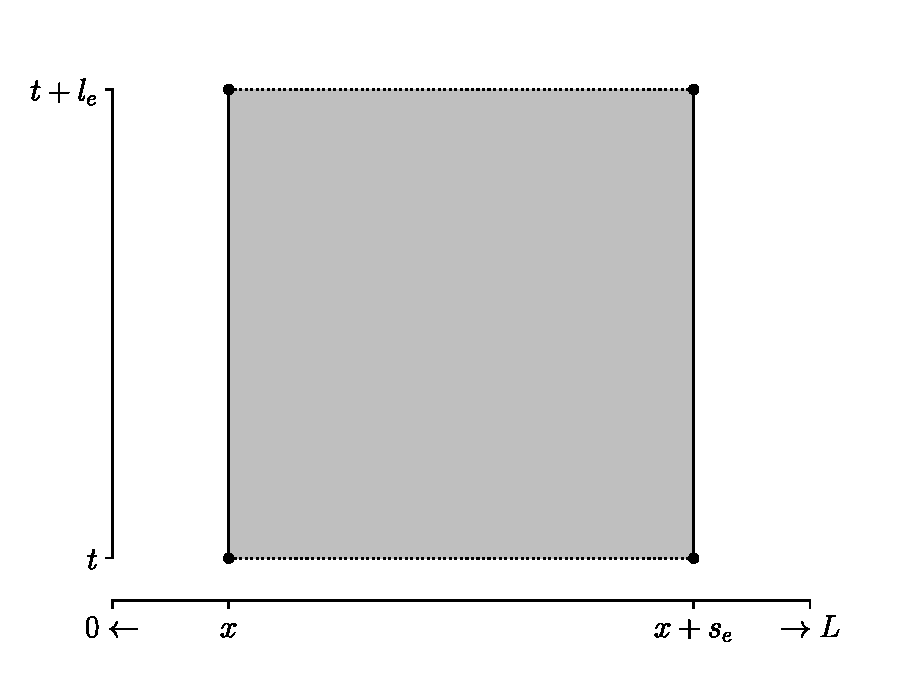
\includegraphics[width=\linewidth,height=5.20833in,keepaspectratio]{slides_files/mediabag/imgs/edge_weight-0.pdf}
\end{center}

\[
\small l_e:\text{ length in time} \quad s_e:\text{ span in base pairs}
\] \begin{center}
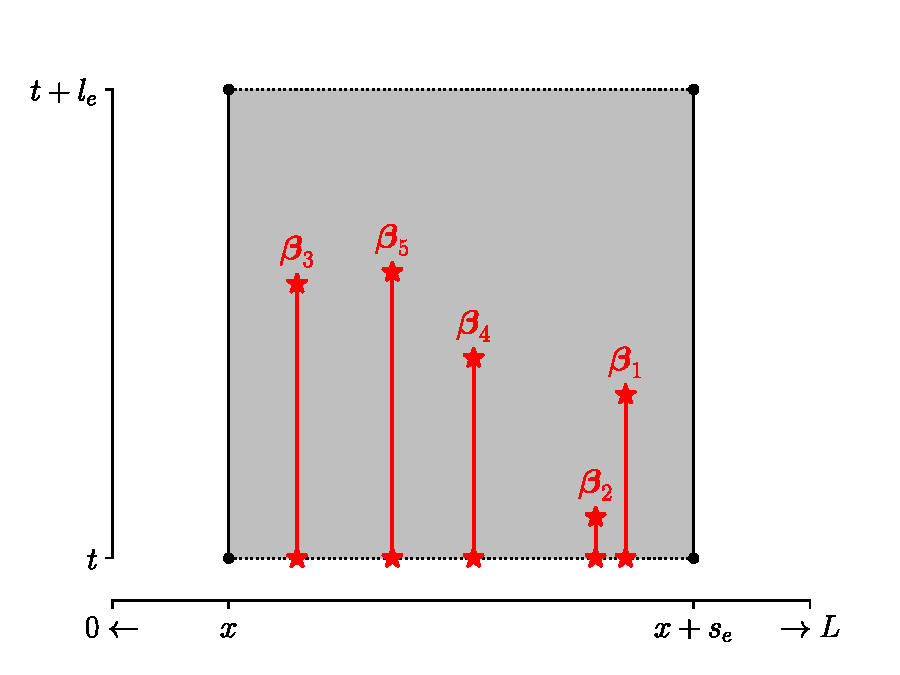
\includegraphics[width=\linewidth,height=5.20833in,keepaspectratio]{slides_files/mediabag/imgs/edge_weight-1.pdf}
\end{center}

\[
\small \mathrm{Var}(\mathbf{u}_e) \quad \propto \quad \text{Number of mutations} \quad \propto \quad \text{Area}=l_es_e
\]

\section{Complex traits through the lens of
ARG-LMM}\label{complex-traits-through-the-lens-of-arg-lmm}

\[
\text{What does ARG-LMM tell us about complex trait analysis?}
\]

\subsection{Genetic value covariance}\label{genetic-value-covariance}

\begin{center}
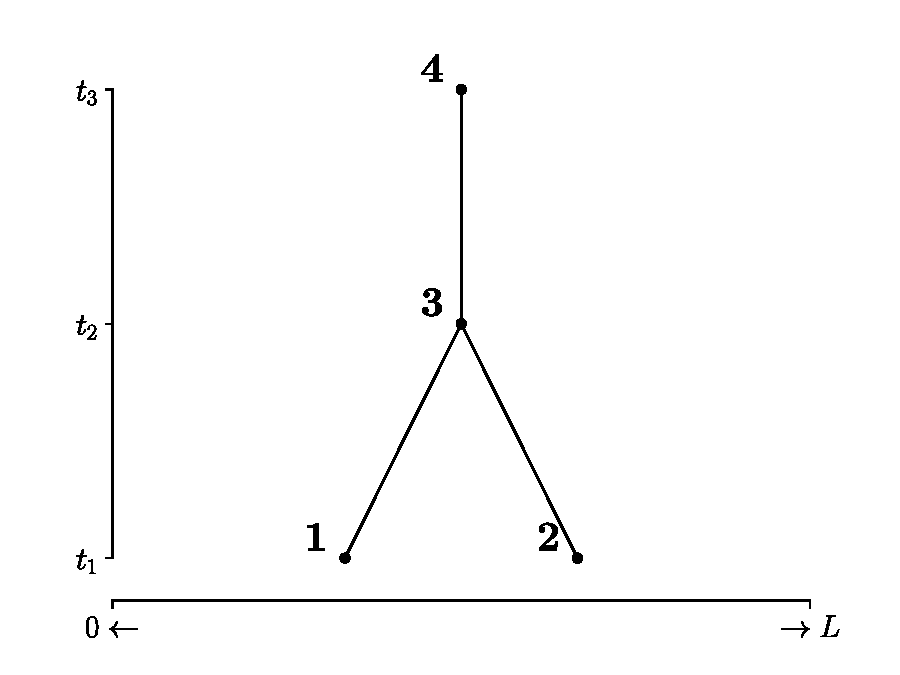
\includegraphics[width=\linewidth,height=6.25in,keepaspectratio]{slides_files/mediabag/imgs/covariance-0.pdf}
\end{center}

\begin{center}
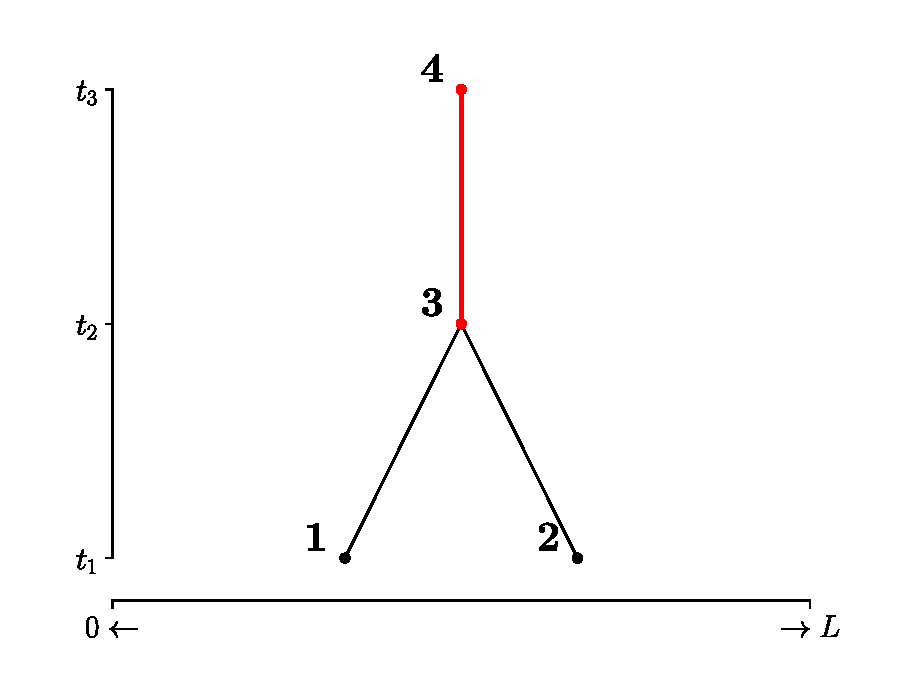
\includegraphics[width=\linewidth,height=6.25in,keepaspectratio]{slides_files/mediabag/imgs/covariance-1.pdf}
\end{center}

\(\mathbf{y}_1 = \mathbf{u}_{13} + \mathbf{u}_{34} \quad \text{and} \quad \mathbf{y}_2 = \mathbf{u}_{23} + \mathbf{u}_{34}\)

\[
\mathrm{Cov}(\mathbf{y}_1, \mathbf{y}_2) = 
\mathrm{Cov}(\mathbf{u}_{13} + \mathbf{u}_{34}, \mathbf{u}_{23} + \mathbf{u}_{34}) =
\mathrm{Cov}(\mathbf{u}_{34}, \mathbf{u}_{34}) =
\mathrm{Var}(\mathbf{u}_{34}) \propto t_3 - t_2
\]

\[
\mathrm{Cov}(\mathbf{y}_1, \mathbf{y}_2) = 
\mathrm{Cov}(\mathbf{u}_{13} + \textcolor{red}{\mathbf{u}_{34}}, \mathbf{u}_{23} + \textcolor{red}{\mathbf{u}_{34}}) =
\mathrm{Cov}(\textcolor{red}{\mathbf{u}_{34}}, \textcolor{red}{\mathbf{u}_{34}}) =
\mathrm{Var}(\textcolor{red}{\mathbf{u}_{34}}) \propto t_3 - t_2
\]

\subsection{\texorpdfstring{Heritability is \emph{ill}-defined in
ARG-LMM}{Heritability is ill-defined in ARG-LMM}}\label{heritability-is-ill-defined-in-arg-lmm}

\[
\small \text{Heritability: }h_g^2 = \frac{\mathrm{Var}(\mathbf{g}_n)}{\mathrm{Var}(\mathbf{y}_n)}
=\frac{\mathrm{Var}(\mathbf{g}_n)}{\mathrm{Var}(\mathbf{g}_n)+\mathrm{Var}(\boldsymbol{\varepsilon}_n)}
\] This applies to all individuals \(\small n \in \{1,\ldots,N\}\)

However, all individuals have a different amount of genetic variance
(except haploids) \[
\small \mathrm{Var}(\mathbf{g}_n) = \mathrm{Var}(\mathbf{h}_{n1}+\mathbf{h}_{n2}) = \mathrm{Var}(\mathbf{h}_{n1}) + \mathrm{Var}(\mathbf{h}_{n2}) + 2\mathrm{Cov}(\mathbf{h}_{n1},\mathbf{h}_{n2})
\]

\[
\small \mathrm{Var}(\mathbf{g}_n) = \mathrm{Var}(\mathbf{h}_{n1}+\mathbf{h}_{n2}) = \mathrm{Var}(\mathbf{h}_{n1}) + \mathrm{Var}(\mathbf{h}_{n2}) + 2\textcolor{red}{\underbrace{\mathrm{Cov}(\mathbf{h}_{n1},\mathbf{h}_{n2})}_{\text{Self-relatedness}}}
\]

We can't define a single quantitity
\(h^2_g=\frac{\textcolor{red}{\mathrm{Var}(\mathbf{g}_n)}}{\textcolor{red}{\mathrm{Var}(\mathbf{g}_n)} + \mathrm{Var}(\boldsymbol{\varepsilon}_n)}\)
for everyone

\begin{center}
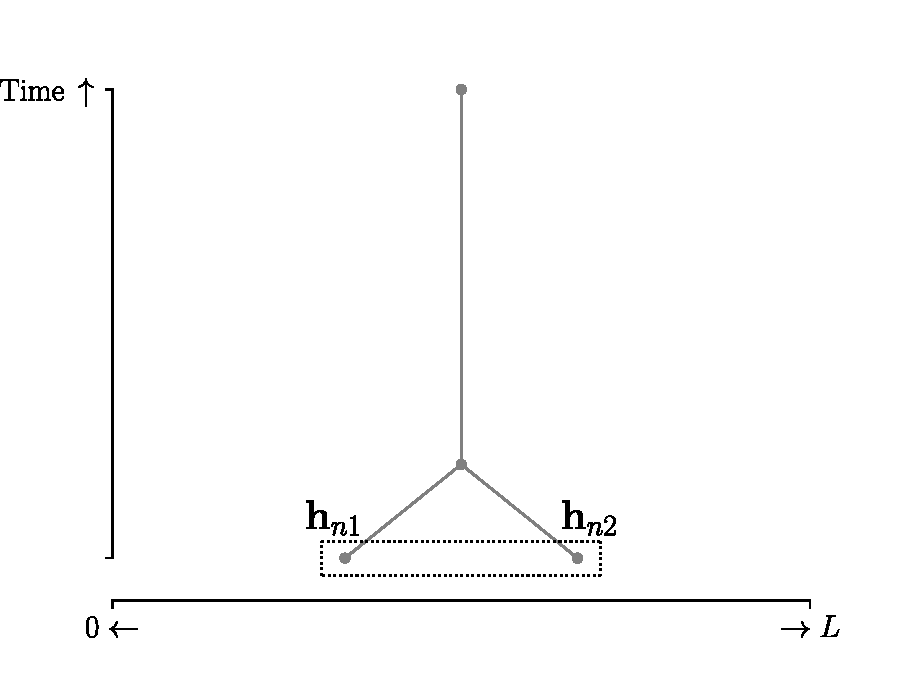
\includegraphics[width=\linewidth,height=5.72917in,keepaspectratio]{slides_files/mediabag/imgs/covariance-short-0.pdf}
\end{center}

\begin{center}
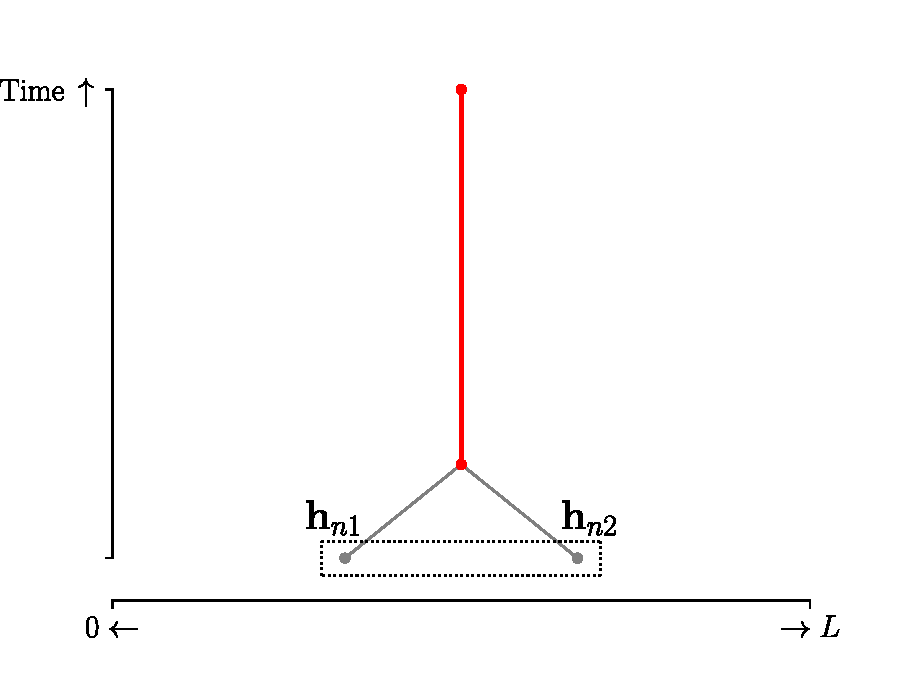
\includegraphics[width=\linewidth,height=5.72917in,keepaspectratio]{slides_files/mediabag/imgs/covariance-short-1.pdf}
\end{center}

\begin{center}
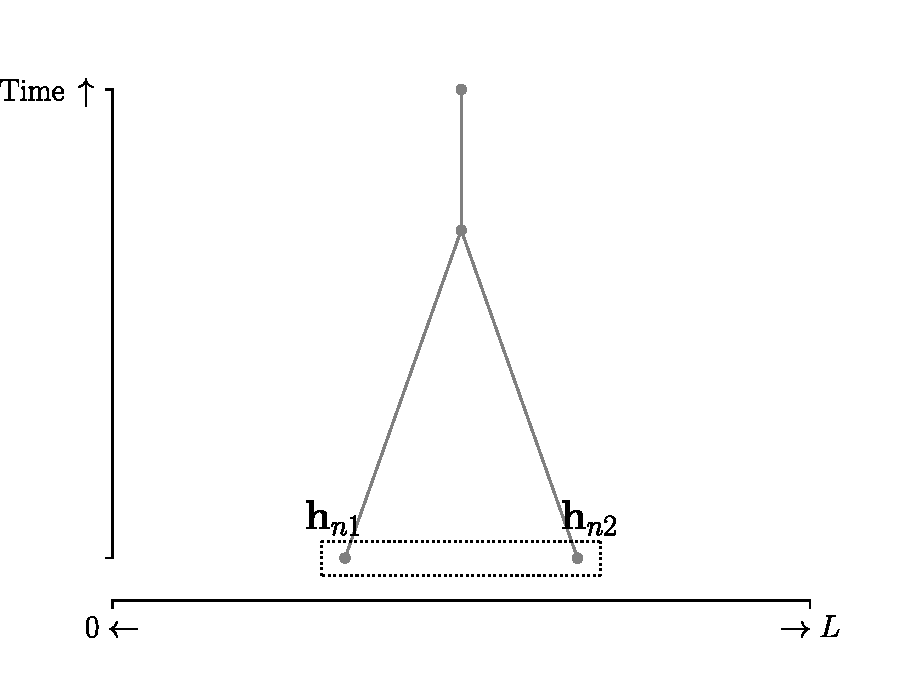
\includegraphics[width=\linewidth,height=5.72917in,keepaspectratio]{slides_files/mediabag/imgs/covariance-long-0.pdf}
\end{center}

\begin{center}
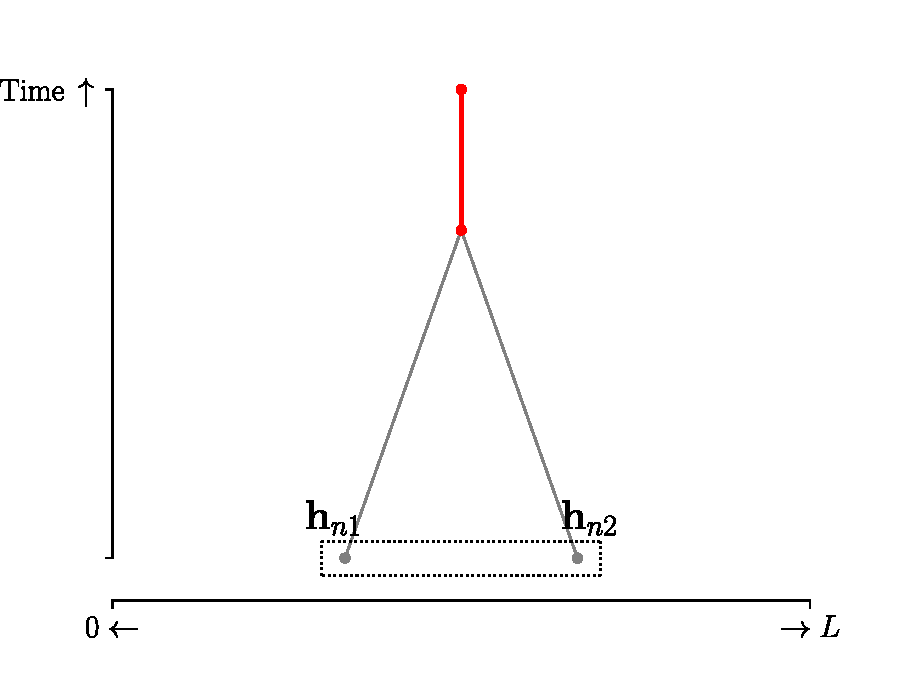
\includegraphics[width=\linewidth,height=5.72917in,keepaspectratio]{slides_files/mediabag/imgs/covariance-long-1.pdf}
\end{center}

\subsection{Polygenic prediction is constrained by
demography}\label{polygenic-prediction-is-constrained-by-demography}

\begin{center}
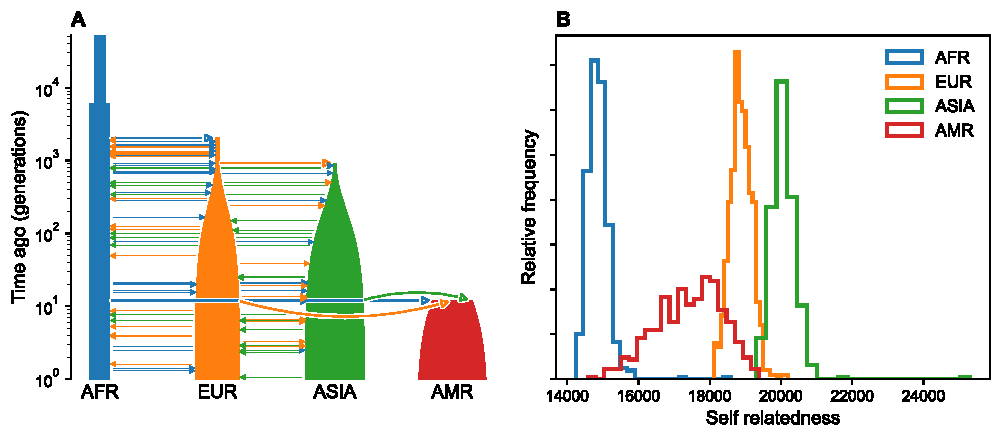
\includegraphics[width=\linewidth,height=5.72917in,keepaspectratio]{slides_files/mediabag/imgs/geneticvariance.pdf}
\end{center}

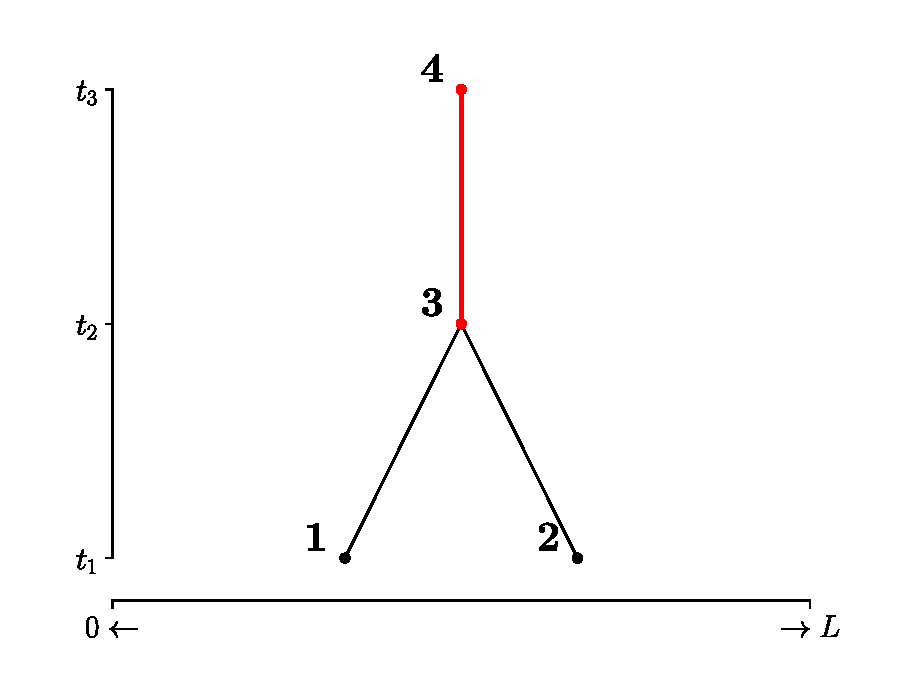
\includegraphics[width=\linewidth,height=5.72917in,keepaspectratio]{slides_files/mediabag/imgs/covariance-1.pdf}

Some people are less genetically variable than others

Some people are harder to predict genetically than others

Some populations are {inherently harder} to predict!

Demographic model from (Browning et al. 2018)

\section{\texorpdfstring{\(\textsf{tslmm}\), fitting ARG-LMM to tree
sequences}{\textbackslash textsf\{tslmm\}, fitting ARG-LMM to tree sequences}}\label{textsftslmm-fitting-arg-lmm-to-tree-sequences}

\(\textsf{tslmm}\) utilizes an efficient \emph{genetic relatedness
matrix - vector product} to fit the restricted maximum likelihood (REML)
objective

It can estimate variance components and compute polygenic scores by best
linear unbiased prediction (BLUP)

\subsection{The matrix-vector product
algorithm}\label{the-matrix-vector-product-algorithm}

\begin{center}
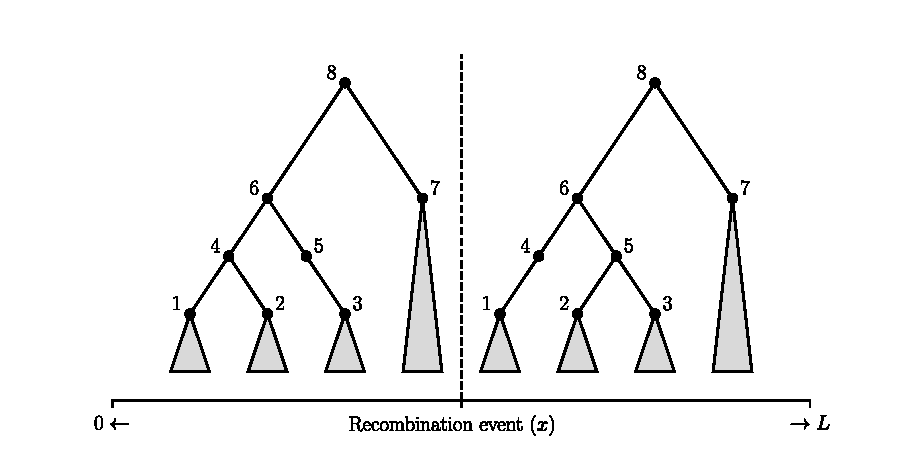
\includegraphics[width=\linewidth,height=5.72917in,keepaspectratio]{slides_files/mediabag/imgs/two-trees-empty.pdf}
\end{center}

\begin{center}
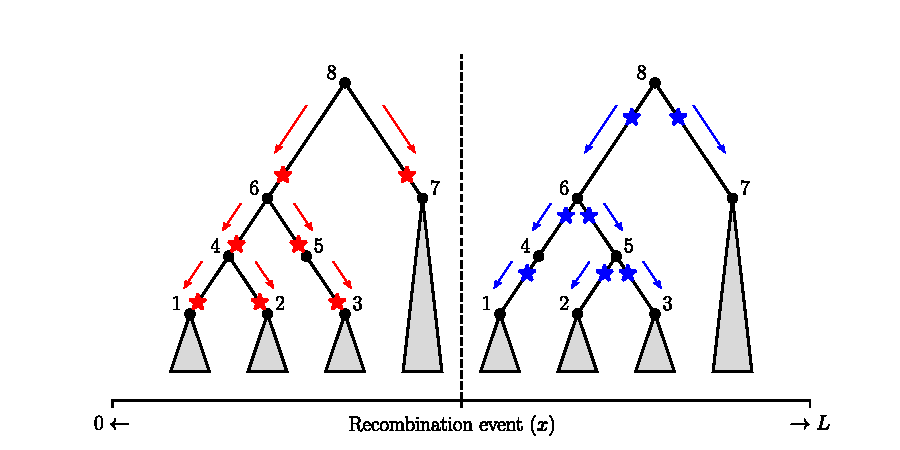
\includegraphics[width=\linewidth,height=5.72917in,keepaspectratio]{slides_files/mediabag/imgs/two-trees-naive.pdf}
\end{center}

\begin{center}
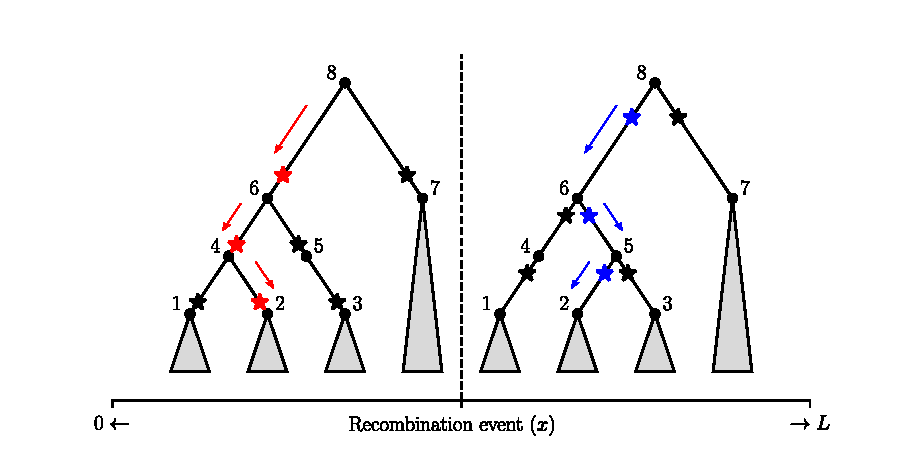
\includegraphics[width=\linewidth,height=5.72917in,keepaspectratio]{slides_files/mediabag/imgs/two-trees-efficient.pdf}
\end{center}

The algorithm needs to pass mutations to the correct samples

A naive approach is to push the mutations down to the leaves every time

Wait until the subtree's topology changes due to edge insertion/deletion

The wrong recipient will receive the mutations if we procrastinate
further

Fitting REML
\(\mathcal{O}(n_s^3) \; \Rightarrow \; \mathcal{O}(n_s+n_t\log n_s)\)

\(n_s\): number of samples, \(n_t\): number of trees

Modified figures by Nathaniel Pope (Oregon)

\subsection{Runtime for variance component
estimation}\label{runtime-for-variance-component-estimation}

\begin{center}
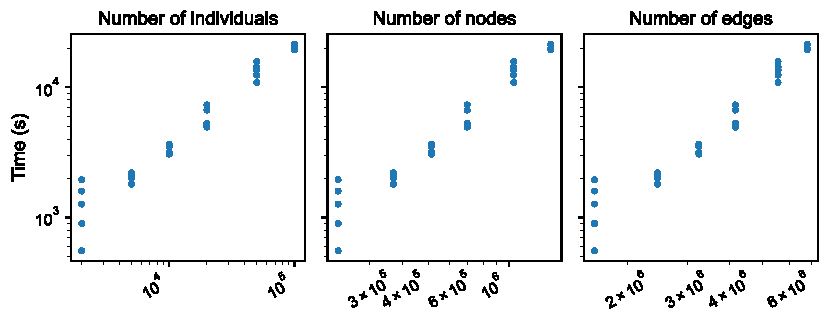
\includegraphics[width=\linewidth,height=5.20833in,keepaspectratio]{slides_files/mediabag/imgs/runtime.pdf}
\end{center}

The runtime scales linearly with respect to the number of individuals
(genome length = \(10^8\))

\subsection{Best linear unbiased prediction
(BLUP)}\label{best-linear-unbiased-prediction-blup}

\begin{center}
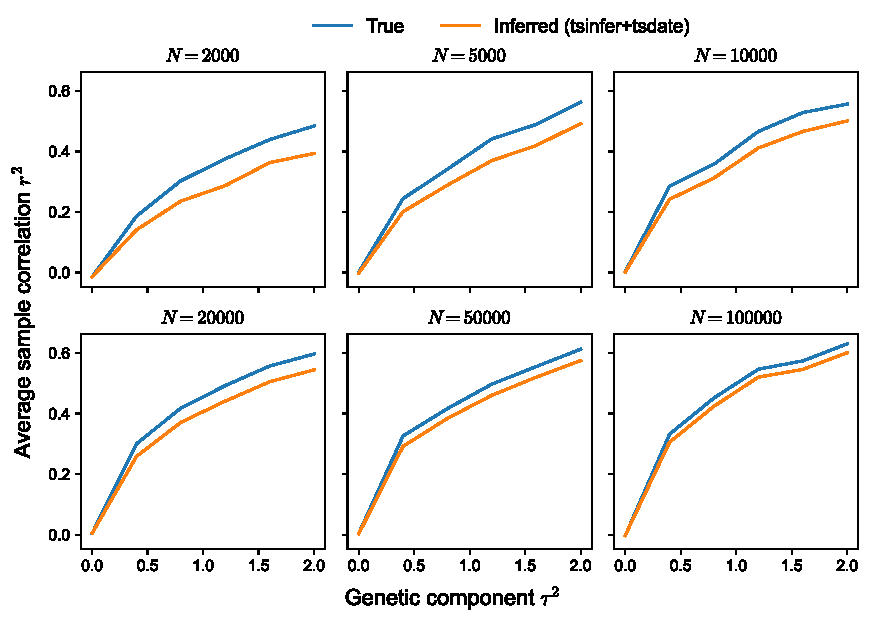
\includegraphics[width=\linewidth,height=6.25in,keepaspectratio]{slides_files/mediabag/imgs/prediction.pdf}
\end{center}

We measured the accuracy of polygenic scores computed from
\(\textsf{tslmm}\)

Training and testing on two non-overlapping groups embedded in the same
tree sequence

True trees are better, but inferred trees are not too behind!

\subsection{Summary \& Future
directions}\label{summary-future-directions}

ARG-LMM lays an explicit connection between population and quantitative
genetics

Pseudoreplication due to shared ancestry (Rosenberg and VanLiere 2009)

Missing heritability, Mutations vs Mendelian segregation

A powerful trait simulator based on ARG-LMM (Cranmer, Brehmer, and
Louppe 2020)

Super interesting technical details and proofs (10+ backup slides
prepared)

Predicting polygenic scores of internal nodes (Edge and Coop 2018; Peng,
Mulder, and Edge 2024)

Time conditioned analysis (random vs fixed effects) (Fan, Mancuso, and
Chiang 2022)

\section{Thank you for listening}\label{thank-you-for-listening}


\includegraphics[width=\linewidth,height=4.16667in,keepaspectratio]{slides_files/mediabag/imgs/qr_code.pdf}

Link to (Lehmann et al. 2025), \(\textsf{tslmm}\) preprint coming soon

Collaborators: Nathaniel Pope (Oregon), Jerome Kelleher (Oxford), Gregor
Gorjanc (Edinburgh), and Peter Ralph (Oregon)

\subsection{References}\label{references}

\phantomsection\label{refs}
\begin{CSLReferences}{1}{0}
\bibitem[\citeproctext]{ref-Browning2018}
Browning, Sharon R., Brian L. Browning, Martha L. Daviglus, Ramon A.
Durazo-Arvizu, Neil Schneiderman, Robert C. Kaplan, and Cathy C. Laurie.
2018. {``Ancestry-Specific Recent Effective Population Size in the
Americas.''} Edited by Kirk E. Lohmueller. \emph{PLOS Genetics} 14 (5):
e1007385. \url{https://doi.org/10.1371/journal.pgen.1007385}.

\bibitem[\citeproctext]{ref-Cranmer2020}
Cranmer, Kyle, Johann Brehmer, and Gilles Louppe. 2020. {``The Frontier
of Simulation-Based Inference.''} \emph{Proceedings of the National
Academy of Sciences} 117 (48): 30055--62.
\url{https://doi.org/10.1073/pnas.1912789117}.

\bibitem[\citeproctext]{ref-Edge2018}
Edge, Michael D, and Graham Coop. 2018. {``Reconstructing the History of
Polygenic Scores Using Coalescent Trees.''} \emph{Genetics} 211 (1):
235--62. \url{https://doi.org/10.1534/genetics.118.301687}.

\bibitem[\citeproctext]{ref-Fan2022}
Fan, Caoqi, Nicholas Mancuso, and Charleston W. K. Chiang. 2022. {``A
Genealogical Estimate of Genetic Relationships.''} \emph{The American
Journal of Human Genetics} 109 (5): 812--24.
\url{https://doi.org/10.1016/j.ajhg.2022.03.016}.

\bibitem[\citeproctext]{ref-Lehmann2025}
Lehmann, Brieuc, Hanbin Lee, Luke Anderson-Trocme, Jerome Kelleher,
Gregor Gorjanc, and Peter L. Ralph. 2025. {``On ARGs, Pedigrees, and
Genetic Relatedness Matrices,''} March.
\url{https://doi.org/10.1101/2025.03.03.641310}.

\bibitem[\citeproctext]{ref-Peng2024}
Peng, Dandan, Obadiah J. Mulder, and Michael D. Edge. 2024.
{``Evaluating ARG-Estimation Methods in the Context of Estimating
Population-Mean Polygenic Score Histories,''} May.
\url{https://doi.org/10.1101/2024.05.24.595829}.

\bibitem[\citeproctext]{ref-Rosenberg2009}
Rosenberg, Noah A., and Jenna M. VanLiere. 2009. {``Replication of
Genetic Associations as Pseudoreplication Due to Shared Genealogy.''}
\emph{Genetic Epidemiology} 33 (6): 479--87.
\url{https://doi.org/10.1002/gepi.20400}.

\bibitem[\citeproctext]{ref-SalehiNowbandegani2023}
Salehi Nowbandegani, Pouria, Anthony Wilder Wohns, Jenna L. Ballard,
Eric S. Lander, Alex Bloemendal, Benjamin M. Neale, and Luke J.
O'Connor. 2023. {``Extremely Sparse Models of Linkage Disequilibrium in
Ancestrally Diverse Association Studies.''} \emph{Nature Genetics} 55
(9): 1494--1502. \url{https://doi.org/10.1038/s41588-023-01487-8}.

\bibitem[\citeproctext]{ref-Wakeley2008}
Wakeley, John. 2008. \emph{Coalescent Theory}. Greenwood Village, CO:
Roberts \& Company.

\bibitem[\citeproctext]{ref-Wong2024}
Wong, Yan, Anastasia Ignatieva, Jere Koskela, Gregor Gorjanc, Anthony W
Wohns, and Jerome Kelleher. 2024. {``A General and Efficient
Representation of Ancestral Recombination Graphs.''} Edited by G Coop.
\emph{GENETICS} 228 (1). \url{https://doi.org/10.1093/genetics/iyae100}.

\bibitem[\citeproctext]{ref-Zhang2023}
Zhang, Brian C., Arjun Biddanda, Árni Freyr Gunnarsson, Fergus Cooper,
and Pier Francesco Palamara. 2023. {``Biobank-Scale Inference of
Ancestral Recombination Graphs Enables Genealogical Analysis of Complex
Traits.''} \emph{Nature Genetics} 55 (5): 768--76.
\url{https://doi.org/10.1038/s41588-023-01379-x}.

\end{CSLReferences}

\section{Technical Notes}\label{technical-notes}

\subsection{Edge splitting}\label{edge-splitting}

\begin{itemize}
\tightlist
\item
  Nodes and edges are reused across multiple trees in a tree sequence
\item
  Edges, in particular, may not have a unique set of samples along their
  span
\item
  Salehi Nowbandegani and colleagues \emph{bricked} the edges to divide
  them (Salehi Nowbandegani et al. 2023)
\item
  Henceforth, we assume that edges are splitted to have a unique
  subtopology \[
  \mathbf{Z}_{ne} = \text{The number of haplotypes of individual $n$ that inherit $e$} 
  \] The overall matrix \(\mathbf{Z}\) is an individual-edge design
  matrix.
\end{itemize}

\subsection{Collapsing variants to
edges}\label{collapsing-variants-to-edges}

\begin{itemize}
\tightlist
\item
  When does an individual possess a derived allele?
  (\(\text{ancestral}=0\), \(\text{derived}=1\))
\item
  Let \(\mathbf{1}_{ep}\) be the indicator \emph{random} variable of a
  mutation at edge \(e\) and position \(p\)
\end{itemize}

An individual should be a descendant of an edge (\(\mathbf{Z}_{ne}=1\))

\[
+
\] That edge should have mutation (\(\mathbf{1}_{ep}=1\))

\[
\mathbf{G}_{np} = \sum_{e: p \in e} \mathbf{Z}_{ne} \mathbf{1}_{ep} \quad \Leftrightarrow \quad \mathbf{G}_p = \sum_{e:p \in e} \mathbf{Z}_{e} \mathbf{1}_{ep}
\]

\begin{itemize}
\tightlist
\item
  Assumes that there are no parent-child mutation pairs, but allows
  \emph{some} recurrent mutations
\end{itemize}

\subsection{Exchange the summations}\label{exchange-the-summations}

Recall
\(\mathbf{G}_p = \sum_{e:p \in e} \mathbf{Z}_{e} \mathbf{1}_{ep}\) and
\(\mathbf{y} = \sum_{p=1}^P \mathbf{G}_p \boldsymbol{\beta}_p + \boldsymbol{\varepsilon}\)

Substitute \(\mathbf{G}_p\) \[
\textcolor{red}{\sum_{p=1}^P \sum_{e:p \in e}} \mathbf{Z}_e \boldsymbol{\beta}_p \mathbf{1}_{ep} + \boldsymbol{\varepsilon}
\]

Exchange the inner and the outer summation \[
\textcolor{red}{\sum_{e=1}^E \sum_{p:p \in e}} \mathbf{Z}_e \boldsymbol{\beta}_p \mathbf{1}_{ep} + \boldsymbol{\varepsilon} 
\]

Pull out \(\mathbf{Z}_e\) and group the positions nested in
\(p: p \in e\) \[
\begin{aligned}
    & \sum_{e=1}^E \mathbf{Z}_e \textcolor{blue}{\left(\sum_{p:p\in e} \boldsymbol{\beta}_p \mathbf{1}_{ep} \right)} + \boldsymbol{\varepsilon} \\
    &= \sum_{e=1}^E \mathbf{Z}_e \textcolor{blue}{\boldsymbol{\upsilon}_e} + \boldsymbol{\varepsilon} \\
    &= \mathbf{Z} \boldsymbol{\upsilon} + \boldsymbol{\varepsilon}
\end{aligned}
\]

\(\boldsymbol{\upsilon}\) is a random variable made up of
mutation-driven random variables \(\mathbf{1}_{ep}\)!

\subsection{Random effects are
independent}\label{random-effects-are-independent}

\begin{itemize}
\item
  Independent entries of random effects is a key assumption of linear
  mixed models
\item
  This can be \emph{proved} in ARG-LMM, instead of assuming it \[
    \mathrm{Cov}( \mathbf{u}_e, \mathbf{u}_{e'} ) = \sum_{p \in e,e'} \boldsymbol{\beta}_p^2 \mathrm{Cov}(\mathbf{1}_{ep}, \mathbf{1}_{e'p})
  \]
\item
  The covariance between the indicators are higher-order terms of
  mutation rates, so we ignore it (Wakeley 2008) \[
    \begin{aligned}
    \mathrm{Cov}(\mathbf{1}_{ep}, \mathbf{1}_{e'p}) &= \mathrm{E}[\mathbf{1}_{ep}\mathbf{1}_{e'p}] - \mathrm{E}[\mathbf{1}_{e'p}]\mathrm{E}[\mathbf{1}_{ep}] \\
        &= 0 -l_eu_{ep}l_{e'}u_{e'p} \approx 0
    \end{aligned}
  \] where \(l_e\) is the (time-)length of edge \(e\).
\end{itemize}

\subsection{\texorpdfstring{The marginal distribution of
\(\mathbf{u}_e\)?}{The marginal distribution of \textbackslash mathbf\{u\}\_e?}}\label{the-marginal-distribution-of-mathbfu_e}

\begin{itemize}
\item
  The Gaussian prior on random effects is a popular choice
\item
  One might be tempted to invoke the central limit theorem to
  \(\mathbf{u}_e\) (sum of indicators) \[
        \mathbf{u}_e \bigg/ \sqrt{l_e s_e} \cdot \sqrt{ \frac{1}{s_e} \sum_{p:p \in e} \boldsymbol{\beta}_p^2 u_{ep} } 
        \rightarrow N(0,1^2) \text{ as } s_e \rightarrow \infty
    \] where \(s_e\) is the span (in base pairs) of edge \(e\)
\item
  The convergence is unlikely to be fast enough given the small value of
  \(\mathbf{E}[\mathbf{1}_{ep}]\) (Berry-Esseen).
\item
  Fortunately, the variance is computable and is \[
        \mathrm{Var}(\mathbf{u}_e) = l_e s_e \cdot \frac{1}{s_e} \sum_{p:p \in e} \boldsymbol{\beta}_p^2 u_{ep}
    \]
\end{itemize}

\subsection{\texorpdfstring{More on
\(\mathrm{Var}(\mathbf{u}_e)\)}{More on \textbackslash mathrm\{Var\}(\textbackslash mathbf\{u\}\_e)}}\label{more-on-mathrmvarmathbfu_e}

\begin{itemize}
\tightlist
\item
  The weight \(\mathrm{Var}(\mathbf{u}_e)\) has two components
\item
  The area \(l_e s_e\)
\item
  Mutation rate-weighted squared average of effect sizes \[
        \tau_e^2 = \frac{1}{s_e} \sum_{p:p \in e} \boldsymbol{\beta}_p^2 u_{ep}
    \]
\item
  As a measure of functional significance, variance components are
  confounded by the area
\end{itemize}

\subsection{Fixed effects are constant under
neutrality}\label{fixed-effects-are-constant-under-neutrality}

\begin{itemize}
\tightlist
\item
  Suppose that \(u_{ep}=u_p\), i.e., the mutation rate is constant
  across edges for a given position
\end{itemize}

\[
\begin{aligned}
    &\left[ \mathbf{Z} \mathbf{f} \right]_n = \sum_{e=1}^E \mathbf{Z}_{ne} \mathbf{E}
    \left[ \sum_{p: p \in e} \boldsymbol{\beta}_p\mathbf{1}_{ep} \right] \\
    \end{aligned}
\]

\[
\sum_{p=1}^P \boldsymbol{\beta}_p u_p 
    \left(
            \sum_{e: p \in e} \mathbf{Z}_{ne} l_e
    \right)
    = \sum_{p=1}^P \boldsymbol{\beta}u_p \cdot 2t_{\mathrm{root},p} = \text{const. resp. to $n$}
\]

\begin{itemize}
\item
  An intercept is enough to account for the fixed effects
  \(\mathbf{Z}\mathbf{f}\) under this condition
\item
  The assumption is standard in neutral settings
\end{itemize}

\[
    \text{\textcolor{red}{Conjecture:} selection $\Rightarrow$ fixed effects?}
\]

\subsection{Becareful of
pseudoreplication}\label{becareful-of-pseudoreplication}

\begin{itemize}
\tightlist
\item
  Non-overlapping samples are not independent
\item
  Everyone shares some amount of mutational history
\item
  Parameter estimates (e.g.~variance components) are correlated
\end{itemize}

\begin{center}
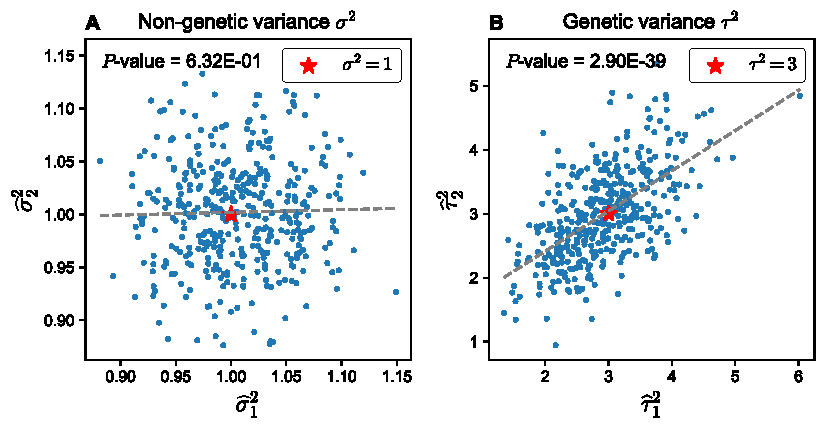
\includegraphics[width=\linewidth,height=4.16667in,keepaspectratio]{slides_files/mediabag/imgs/pseudoreplication.pdf}
\end{center}

This is also the very reason why BLUP works

We are all correlated!

\subsection{\texorpdfstring{\emph{Missing}
heritability?}{Missing heritability?}}\label{missing-heritability}

ARG-LMM variance component only reflects mutational variability

\begin{itemize}
\tightlist
\item
  Pedigree-based heritability captures Mendelian segregation and
  mutation is ignored
\item
  ARG-LMM's generative model only has mutation and no segregation
\item
  Why compare quantities stemming from different random forces? (Zhang
  et al. 2023)
\end{itemize}

\begin{center}

\includegraphics[width=\linewidth,height=4.16667in,keepaspectratio]{slides_files/mediabag/applesandoranges-lil.jpg}
\end{center}

Figure from \href{https://whalebonemag.com/}{Whalebone Magazine}

\subsection{Estimation quality of variance
components}\label{estimation-quality-of-variance-components}

\textbf{Simulated trees}

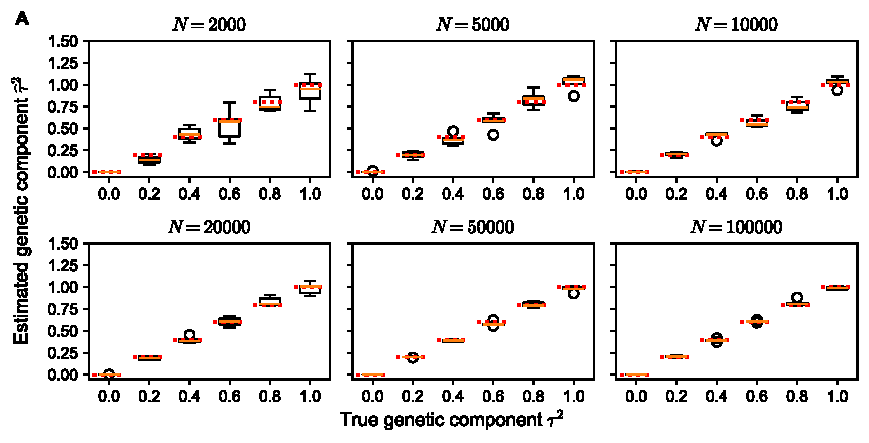
\includegraphics[width=\linewidth,height=7.29167in,keepaspectratio]{slides_files/mediabag/imgs/estimation_true.pdf}

\textbf{Inferred (tsinfer+tsdate) trees}

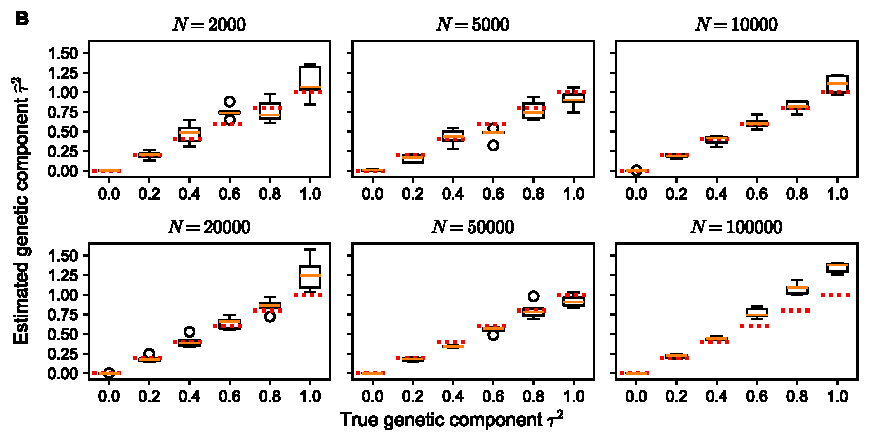
\includegraphics[width=\linewidth,height=7.29167in,keepaspectratio]{slides_files/mediabag/imgs/estimation_infer.pdf}

\subsection{There are many genetic
variances}\label{there-are-many-genetic-variances}

\begin{itemize}
\tightlist
\item
  ARG-conditioned variance \[
  \mathrm{Var}(\mathbf{y} \mid \mathrm{ARG})
  \]
\item
  Pedigree-conditioned variance \[
  \mathrm{Var}(\mathbf{y} \mid \mathrm{Pedigree})
  \]
\item
  Demography-conditioned variance \[
  \mathrm{Var}(\mathbf{y} \mid \mathrm{Demography})
  \]
\item
  Time conditioning (reference population)
\end{itemize}




\end{document}
